\chapter[Sistema de reconocimiento y recolección]{Sistema de reconocimiento por visión de maduración de frutos\\
  para su recolección con un brazo robótico}
\label{cap:capitulo5}

La automatización de tareas agrícolas mediante tecnologías de visión artificial es una línea de investigación en plena expansión, especialmente en lo que respecta a la cosecha de productos delicados como las frutas, y más concretamente, las fresas. La maduración irregular, la variabilidad del entorno y la necesidad de recolección selectiva representan retos importantes, por lo que este proyecto nace con el propósito de aportar una solución basada en visión artificial y robótica colaborativa que permita mejorar la eficiencia y precisión en la recolección, reduciendo la intervención humana y el riesgo de daños al fruto.\\

El presente Trabajo de Fin de Grado se enmarca en el desarrollo de un sistema de visión por ordenador para la detección de fresass maduras, con el objetivo de facilitar su recolección mediante un brazo robótico de la marca Universal Robots (UR). Este sistema propuesto permite detectar visualmente las fresas y estimar su posición en el espacio tridimensional utilizando una única cámara, integrando los datos en tiempo real con el robot colaborativo para ejecutar tareas de recolección automática.

\section{Hipótesis suelo adaptada al plano vertical}
\label{sec:HS_vertical}

El sistema propuesto se basa en la estimación de coordenadas tridimensionales a partir de una única cámara RGB fija, por lo que, para poder realizar esta estimación sin recurrir a sensores adicionales, se ha adoptado la hipótesis del suelo, una técnica habitual en visión por computador que asume que los objetos de interés se encuentran sobre un plano conocido y fijo respecto a la cámara.\\

La hipótesis suelo (Figura \ref{fig:HS} tomada del artículo \cite{Vega21}) supone que todos los objetos del mundo en 3D están apoyados sobre el suelo, por lo tanto, asumiendo que el suelo está en el plano Z = 0, nos permitirá estimar, con una única cámara, la posición 3D de los puntos que estén en el suelo.

\begin{figure} [H]
    \begin{center}
      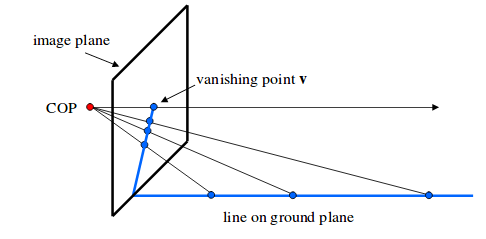
\includegraphics[width=9cm]{figs/Hipotesis suelo.png}
    \end{center}
    \caption{La hipótesis suelo asume que todos los objetos están en el suelo}
    \label{fig:HS}
\end{figure}

En este caso, y debido a la orientación del escenario, la hipótesis ha sido adaptada al plano vertical, lo que significa que se asume que las fresas están dispuestos sobre una superficie vertical, como es el caso en los huertos verticales, cuya distancia a la cámara es constante. Esta modificación permite proyectar los puntos detectados en la imagen 2D al espacio 3D, siempre que se disponga de los parámetros intrínsecos de la cámara y se conozca la geometría del plano.

Durante la calibración del sistema se ha definido un plano de trabajo vertical, y se ha establecido un sistema de coordenadas 3D cuyo origen coincide con el punto central de la imagen proyectada por la cámara sobre ese plano, actuando como referencia para crear el plano común a través de la interfaz del robot con las mismas orientaciones de los ejes de coordenadas que la propia brida de herramienta del UR (Figura \ref{fig:Plano_pared_UR}), y que permite calcular las coordenadas relativas de las fresas detectadas y calcular la distancia a cada detección proyectando el centro del \textit{bounding box} sobre el plano vertical y usando la matriz de calibración de la cámara. 

\begin{figure} [H]
    \begin{center}
      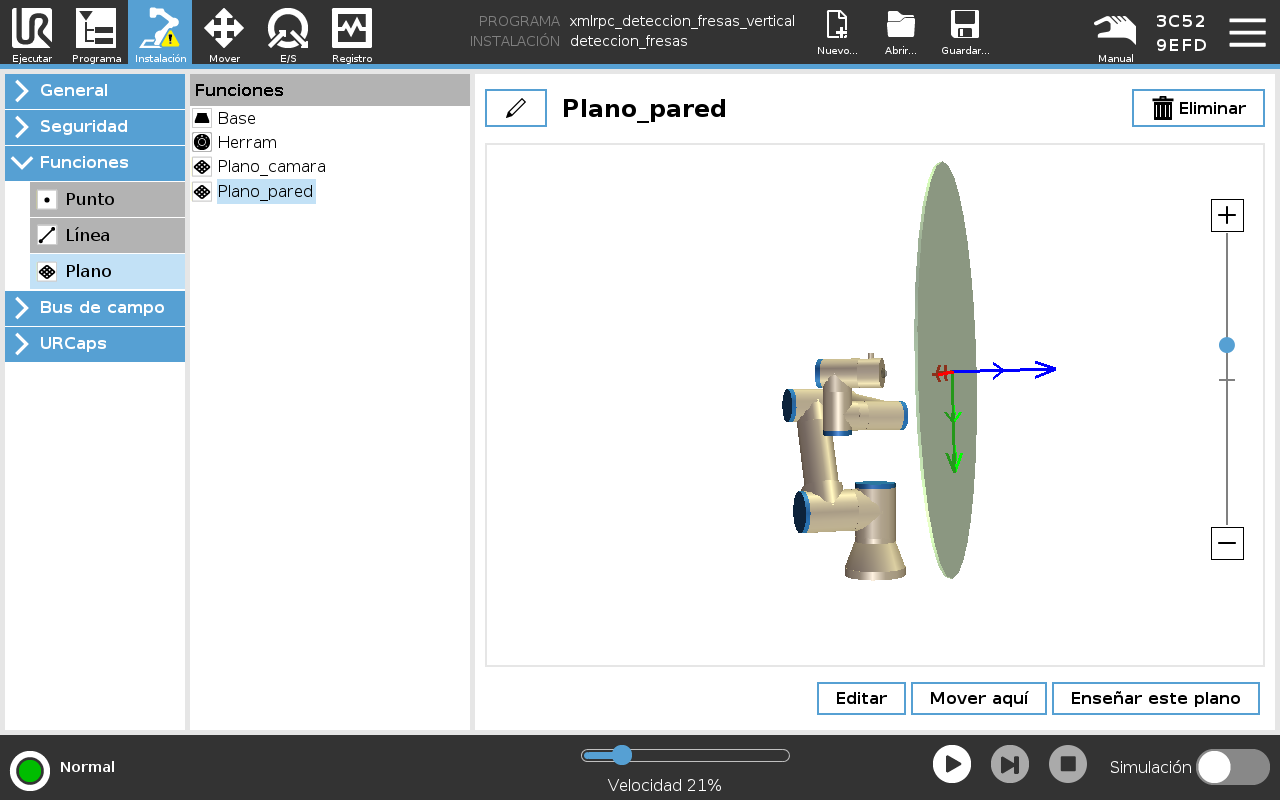
\includegraphics[width=14cm]{figs/Plano Pared Programa UR.png}
    \end{center}
    \caption{Plano pared generado en el UR}
    \label{fig:Plano_pared_UR}
\end{figure}

\section{Técnica de visión}
\label{sec:Tecnica_Vision}

La detección de las fresas maduras se ha resuelto mediante el uso de técnicas de visión artificial basadas en deep learning, concretamente, se ha utilizado el modelo YOLOv3 (You Only Look Once), un detector de objetos en tiempo real ampliamente utilizado por su equilibrio entre precisión y velocidad.\\

Este modelo ha sido entrenado específicamente para reconocer fresas maduras en las condiciones del entorno de trabajo, y una vez entrenado, se ha integrado en un script que analiza el flujo de vídeo en tiempo real y devuelve las coordenadas de cada objeto detectado en la imagen 2D, junto con la clase del objeto y la confianza de detección. Para mejorar la precisión en la estimación de la posición, se ha utilizado el centro del \textit{bounding box} de la fresa detectada como punto de referencia para la proyección sobre el plano vertical, conforme a la hipótesis descrita en el apartado anterior.\\

La comunicación entre el módulo de visión y el robot se realiza mediante XML-RPC, un protocolo ligero y eficiente que permite establecer una conexión entre el programa que corre en el ordenador y el robot UR, siendo el servidor quién transmite al robot las coordenadas tridimensionales de las detecciones, permitiendo una integración fluida en tiempo real. 

\section{Modelo de hardware utilizado e integración con el robot}
\label{sec:modelo_HW}

El sistema completo se ha implementado utilizando una combinación de componentes hardware específicos que permiten tanto la detección como la ejecución de la acción robótica, y que se encuentran descritos en el Capítulo \ref{cap:capitulo4}, siendo el proceso completo de integración el siguiente:

\begin{itemize}
  \item La cámara captura imágenes de la escena en tiempo real.
  \item El modelo de deep learning detecta las fresas maduras y genera sus posiciones en píxeles.
  \item Estas coordenadas se proyectan al espacio 3D sobre el plano vertical.
  \item El servidor XML-RPC transmite las coordenadas al robot UR.
  \item El robot interpreta la posición, calcula una trayectoria y actúa sobre la fruta detectada.
\end{itemize}

Esta arquitectura permite un sistema modular, robusto y fácilmente escalable a escenarios reales más complejos, sentando las bases para su posible aplicación futura en entornos agrícolas reales o semiautomatizados, y para conseguir la cuál deben seguirse los siguientes pasos de forma ordenada si se desea conseguir una correcta integración entre el sistema de visión y el brazo robótico UR.

\begin{enumerate}
  \item Conexión de red: En primer lugar, es fundamental asegurarse de que tanto el robot como el ordenador que ejecuta el sistema de visión están conectados a la misma red local, y se recomienda usar conexión por cable para mayor estabilidad. Es necesario comprobar que hay conectividad entre ambos dispositivos (por ejemplo, mediante un ping a la IP del robot desde el ordenador), ya que la comunicación se establece a través del protocolo XML-RPC sobre una dirección IP y puerto determinados.
  \item Definición de la Instalación del robot: Si el robot lleva instalada una herramienta, como una garra o un actuador, es importante configurar correctamente la carga útil, el peso y el centro de gravedad en el software del UR, ya que esto garantiza un funcionamiento seguro y preciso, ajustando los parámetros de control de movimiento y compensación de la cinemática.
  \item Creación del plano de trabajo: A continuación, se debe definir el plano de trabajo sobre el que se va a operar, en este caso un plano vertical, como se detalló en la sección \ref{sec:HS_vertical}. 
  \item Lanzamiento del sistema de comunicación: Posteriormente, se debe ejecutar el script Python que ejerce de servidor desde la terminal del ordenador, para poder ejecutar el programa en el UR que realiza la solicitud de datos al servidor remoto a través del protocolo XML-RPC, una vez que el servidor esté en marcha.
  \item Ejecución: Una vez en marcha, el sistema detectará automáticamente las fresas presentes en la escena, calculará sus coordenadas tridimensionales y las enviará al robot, que ejecutará el movimiento correspondiente para acercarse al fruto y proceder a su recolección.
\end{enumerate}

\vspace{20mm}

Con todo lo anterior, se ha descrito en detalle el sistema desarrollado, incluyendo los fundamentos técnicos, las herramientas de visión artificial empleadas, y el proceso de integración con el robot colaborativo UR, siendo un sistema diseñado con el objetivo de ser modular, reproducible y eficaz en tareas de detección y recolección de frutos maduros en entornos controlados. A continuación, en el siguiente capítulo, se presentan los experimentos realizados, donde se detallan las diferentes pruebas llevadas a cabo, los ajustes realizados durante el desarrollo y los resultados obtenidos hasta alcanzar el estado funcional final del proyecto.

















